\section{Test Description and Success Criteria}
The tests are located in \texttt{simulation/dynamics/VSCMGs/\_UnitTest/\newline
test\_VSCMGStateEffector\_integrated.py} \textbf{and} \texttt{simulation/dynamics/VSCMGs/\newline\_UnitTest/
test\_VSCMGStateEffector\_ConfigureVSCMGRequests.py}. Depending on the test, there are different success criteria. These are outlined in the following subsections:
\subsection{Balanced Wheels Scenario - Integrated Test}
In this test the simulation is placed into orbit around Earth with point gravity, has 3 VSCMGs attached to the spacecraft, and they are in ``Balanced Wheels" mode. The following parameters are being tested:
\begin{itemize}
	\item Conservation of orbital angular momentum
	\item Conservation of orbital energy
	\item Conservation of rotational angular momentum
	\item Conservation of rotational energy
	\item Achieving the expected final attitude
	\item Achieving the expected final position
\end{itemize}

\subsection{Simple Jitter Scenario - Integrated Test}
In this test the simulation is placed into orbit around Earth with point gravity, has 3 VSCMGs attached to the spacecraft, and they are in ``Simple Jitter" mode. The following parameters are being tested:
\begin{itemize}
\item Achieving the expected final attitude
\item Achieving the expected final position
\end{itemize}

\subsection{Fully Coupled Jitter Scenario without Gravity - Integrated Test}
In this test the simulation 3 VSCMGs are attached to the spacecraft, and they are in ``Fully Coupled Jitter" mode.  The following parameters are being tested:
\begin{itemize}
\item Conservation of orbital angular momentum
\item Conservation of orbital energy
\item Conservation of rotational angular momentum
\item Conservation of rotational energy
\item Achieving the expected final attitude
\item Achieving the expected final position
\end{itemize}

\subsection{Fully Coupled Jitter Scenario  with Gravity- Integrated Test}
In this test the simulation is placed into orbit around Earth with point gravity, has 3 VSCMGs attached to the spacecraft, and they are in ``Fully Coupled Jitter Gravity" mode. The following parameters are being tested:
\begin{itemize}
\item Conservation of orbital angular momentum
\item Conservation of orbital energy
\item Conservation of rotational angular momentum
\item Achieving the expected final attitude
\item Achieving the expected final position
\end{itemize}

\section{Test Parameters}

Since this is an integrated test, the inputs to the test are the physical parameters of the spacecraft along with the initial conditions of the states. These parameters are outlined in Tables~\ref{tab:hub}-~\ref{tab:initial}. Additionally, the error tolerances can be seen in Table~\ref{tab:errortol}. The energy-momentum conservation values will normally have an agreement down to 1e-14, but to ensure cross-platform agreement the tolerance was chose to be 1e-10. The position and attitude checks have a tolerance set to 1e-7 and is because 8 significant digits were chosen as the values being compared to. 

\begin{table}[htbp]
	\caption{Spacecraft Hub Parameters for Energy Momentum Conservation Scenarios}
	\label{tab:hub}
	\centering \fontsize{10}{10}\selectfont
	\begin{tabular}{ c | c | c | c } % Column formatting, 
		\hline
		\textbf{Name}  & \textbf{Description}  & \textbf{Value} & \textbf{Units} \\
		\hline
		mHub  & mass & 750.0 & kg \\
		IHubPntBc\_B & Inertia in $\cal{B}$ frame & $\begin{bmatrix}
		900.0 & 0.0 & 0.0\\
		0.0 & 800.0 & 0.0\\
		0.0 & 0.0 & 600.0
		\end{bmatrix}$ & kg-m$^2$ \\
		r\_BcB\_B & CoM Location in $\cal{B}$ frame & $\begin{bmatrix}
		-0.0002 & 0.0001 & 0.1 \end{bmatrix}^T$ & m \\
		sigma\_BNInit & Initial MRP of $\cal{B}$ frame & $\begin{bmatrix}
		0.0 & 0.0 & 0.0
		\end{bmatrix}^T$ & - \\
		omega\_BN\_BInit & Initial Angular Velocity of $\cal{B}$ frame & $			
		\begin{bmatrix}
		0.08 & & 0.01 & 0.0
		\end{bmatrix}^T$ & rad/s \\
		\hline
	\end{tabular}
\end{table}

\begin{table}[htbp]
	\caption{VSCMG Parameters Across All Tests}
	\label{tab:rw15}
	\centering \fontsize{10}{10}\selectfont
	\begin{tabular}{ c | c | c | c } % Column formatting, 
		\hline
		\textbf{Name}  & \textbf{Description}  & \textbf{Value} & \textbf{Units} \\
		\hline
		Js  & Spin Axis Inertia & 0.159 & kg-m$^2$ \\
		mass & mass & 12.0 & kg \\
		U\_s & Static Imbalance & 4.8E-6 & kg-m \\
		U\_d & Dynamic Imbalance & 15.4E-7 & kg-m$^2$ \\
		Omega\_max & Max Wheel Speed & 628.32 & rad/s \\
		IW1 & Spin Axis $\hat{w_1}$ Rotor Moment of Inertia & 0.159  & kg-m$^2$ \\
		IW2 &  $\hat{w_2}$ Rotor Moment of Inertia & 0.079 & kg-m$^2$ \\
		IW3 & $\hat{w_3}$ Rotor Moment of Inertia & 0.079 & kg-m$^2$ \\
		IG1 & Spin Axis $\hat{g_s}$ Rotor Moment of Inertia & 0.1 & kg-$^2$ \\
		IG2 & $\hat{g_t}$ Rotor Moment of Inertia & 0.2 & kg-m$^2$ \\
		IG3 & $\hat{g_g}$ Rotor Moment of Inertia & 0.3 & kg-m$^2$ \\
		l  & Transverse Offset & 0.01 & m \\
		L & Axial Offset & 0.1 & m \\
		gamma & Gimbal Angle & 0.0  & rad \\
		rGcG\_G & Gimbal Center of Mass in the $\cal{G}$ Frame & $\begin{bmatrix}
		0.0001 & -0.02 & 0.1 \end{bmatrix}^T$ & m \\
		
	\end{tabular}
\end{table}

\begin{table}[htbp]
	\caption{VSCMG 1 Parameters Across All Tests}
	\label{tab:rw12}
	\centering \fontsize{10}{10}\selectfont
	\begin{tabular}{ c | c | c | c } % Column formatting, 
		\hline
		\textbf{Name}  & \textbf{Description}  & \textbf{Value} & \textbf{Units} \\
		\hline
		gsHat0\_B &  $\hat{g_s}_0$ & $\begin{bmatrix}
		1.0 & 0.0 & 0.0 \end{bmatrix}^T$ & \\
		gtHat0\_B &  $\hat{g_t}_0$ & $\begin{bmatrix}
		0.0 & 1.0 & 0.0 \end{bmatrix}^T$ & \\
		ggHat\_B &  $\hat{g_g}_0$ & $\begin{bmatrix}
		0.0 & 0.0 & 1.0 \end{bmatrix}^T$ & \\
		Omega & Initial Wheel Speed & 209.44 & rad/s \\
		gammaDot & Gimbal Rate & 0.06 & rad/s\\
		rGB\_B & Position Vector of the VSCMG in the $\cal{B}$ frame & $\begin{bmatrix}
		0.1& 0.002 & -0.02 \end{bmatrix}^T$ & m \\
		\hline
	\end{tabular}
\end{table}

\begin{table}[htbp]
	\caption{VSCMG 2 Parameters Across All Tests}
	\label{tab:rw13}
	\centering \fontsize{10}{10}\selectfont
	\begin{tabular}{ c | c | c | c } % Column formatting, 
		\hline
		\textbf{Name}  & \textbf{Description}  & \textbf{Value} & \textbf{Units} \\
		\hline
		gsHat0\_B &  $\hat{g_s}_0$ & $\begin{bmatrix}
		0.0 & 1.0 & 0.0 \end{bmatrix}^T$ & \\
		gtHat0\_B &  $\hat{g_t}_0$ & $\begin{bmatrix}
		-0.817 & 0.0 & 0.577 \end{bmatrix}^T$ & \\
		ggHat\_B &  $\hat{g_g}_0$ & $\begin{bmatrix}
		0.577 & 0.0 & 0.817 \end{bmatrix}^T$ & \\
		Omega & Initial Wheel Speed & 36.65 & rad/s \\
		gammaDot & Gimbal Rate & 0.011 & rad/s\\
		rGB\_B & Position Vector of the VSCMG in the $\cal{B}$ frame & $\begin{bmatrix}
		0.0& -0.05 & -0.0 \end{bmatrix}^T$ & m \\
		\hline
	\end{tabular}
\end{table}

\begin{table}[htbp]
	\caption{VSCMG 3 Parameters Across All Tests}
	\label{tab:rw14}
	\centering \fontsize{10}{10}\selectfont
	\begin{tabular}{ c | c | c | c } % Column formatting, 
		\hline
		\textbf{Name}  & \textbf{Description}  & \textbf{Value} & \textbf{Units} \\
		\hline
		gsHat0\_B &  $\hat{g_s}_0$ & $\begin{bmatrix}
		0.0 & 0.0 & 1.0 \end{bmatrix}^T$ & \\
		gtHat0\_B &  $\hat{g_t}_0$ & $\begin{bmatrix}
		0.817 & 0.0 & 0.577 \end{bmatrix}^T$ & \\
		ggHat\_B &  $\hat{g_g}_0$ & $\begin{bmatrix}
		-0.577 & 0.0 & 0.817 \end{bmatrix}^T$ & \\
		Omega & Initial Wheel Speed & -94.25 & rad/s \\
		gammaDot & Gimbal Rate & -0.003 & rad/s\\
		rGB\_B & Position Vector of the VSCMG in the $\cal{B}$ frame & $\begin{bmatrix}
		-0.1 & 0.05 & 0.05 \end{bmatrix}^T$ & m \\
		\hline
	\end{tabular}
\end{table}

\begin{table}[htbp]
	\caption{Initial Conditions for Fully-Coupled Jitter Scenario with Gravity}
	\label{tab:initial}
	\centering \fontsize{10}{10}\selectfont
	\begin{tabular}{ c | c | c | c } % Column formatting, 
		\hline
		\textbf{Name}  & \textbf{Description}  & \textbf{Value} & \textbf{Units} \\
		\hline
		r\_CN\_NInit & Initial Position of S/C & $\begin{bmatrix}
		-4020339 &	7490567 & 5248299 
		\end{bmatrix}^T$ & m \\
		v\_CN\_NInit & Initial Velocity of S/C & $\begin{bmatrix}
		-5199.78 & -3436.68 & 1041.58
		\end{bmatrix}^T$ & m/s \\
		\hline
	\end{tabular}
\end{table}

\begin{table}[htbp]
	\caption{Initial Conditions for Fully-Coupled Jitter Scenario without Gravity}
	\label{tab:initial2}
	\centering \fontsize{10}{10}\selectfont
	\begin{tabular}{ c | c | c | c } % Column formatting, 
		\hline
		\textbf{Name}  & \textbf{Description}  & \textbf{Value} & \textbf{Units} \\
		\hline
		r\_CN\_NInit & Initial Position of S/C & $\begin{bmatrix}
		0.1 &	-0.2 & 0.3
		\end{bmatrix}^T$ & m \\
		v\_CN\_NInit & Initial Velocity of S/C & $\begin{bmatrix}
		-0.4 & -0.5 & -0.8
		\end{bmatrix}^T$ & m/s \\
		\hline
	\end{tabular}
\end{table}

\begin{table}[htbp]
	\caption{VSCMG Wheel and Gimbal Torque for Simple Jitter and Fully-Coupled Jitter Scenario without Gravity Scenarios}
	\label{tab:initial3}
	\centering \fontsize{10}{10}\selectfont
	\begin{tabular}{ c | c | c | c } % Column formatting, 
		\hline
		\textbf{Name}  & \textbf{Description}  & \textbf{Value} & \textbf{Units} \\
		\hline
		wheelTorque & Torque on VSCMG Wheel & $\begin{bmatrix}
		0.001 &	 0.005 & -0.009
		\end{bmatrix}^T$ & N-m \\
		gimbalTorque & Torque on VSCMG Gimbal & $\begin{bmatrix}
		0.008 & -0.0015 & -0.006
		\end{bmatrix}^T$ & N-m \\
		\hline
	\end{tabular}
\end{table}

\begin{table}[htbp]
	\caption{Error Tolerance - Note: Relative Tolerance is $\textnormal{abs}(\frac{\textnormal{truth} - \textnormal{value}}{\textnormal{truth}}$)}
	\label{tab:errortol}
	\centering \fontsize{10}{10}\selectfont
	\begin{tabular}{| c | c |} % Column formatting, 
		\hline
		Test   & Relative Tolerance \\
		\hline
		Energy and Momentum Conservation & 1e-10 \\
		\hline
		Position, Attitude Check & 1e-7 \\
		\hline	
	\end{tabular}
\end{table}

\clearpage

\section{Test Results}

\subsection{Balanced Wheels Scenario - Integrated Test Plots}

\begin{figure}[htbp]\centerline{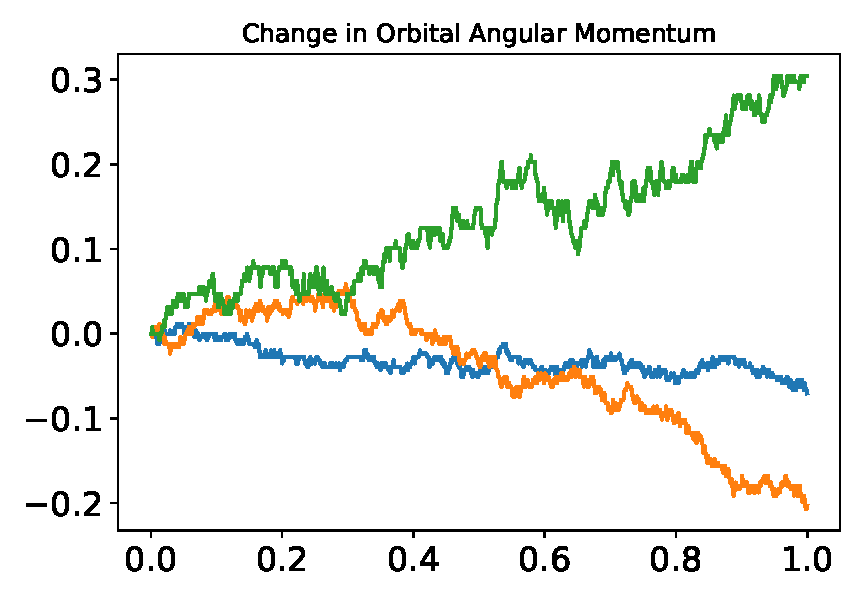
\includegraphics[width=0.80\textwidth]{AutoTeX/ChangeInOrbitalAngularMomentumBalancedWheels}}\caption{Change in Orbital Angular Momentum BalancedWheels}\label{fig:ChangeInOrbitalAngularMomentumBalancedWheels}\end{figure}
\begin{figure}[htbp]\centerline{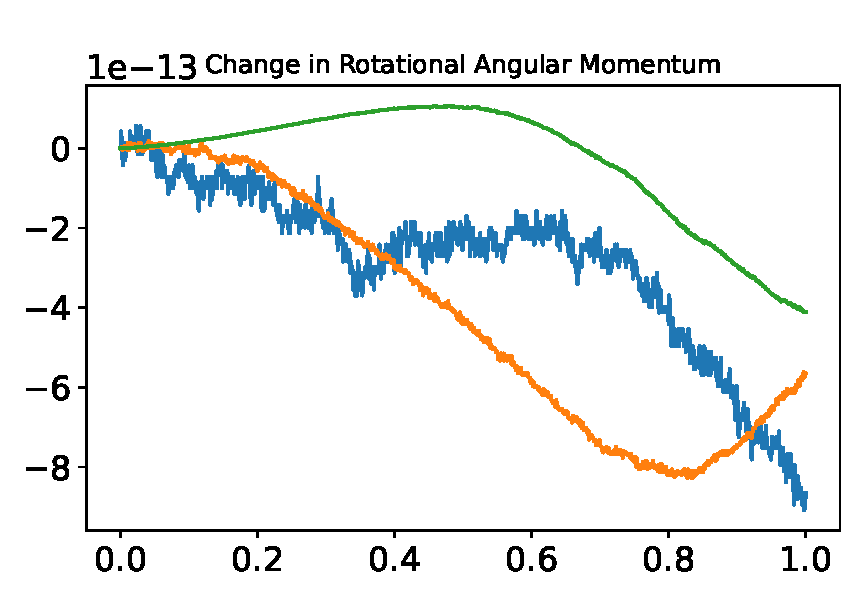
\includegraphics[width=0.8\textwidth]{AutoTeX/ChangeInOrbitalEnergyBalancedWheels}}\caption{Change in Orbital Energy BalancedWheels}\label{fig:ChangeInOrbitalEnergyBalancedWheels}\end{figure}
\begin{figure}[htbp]\centerline{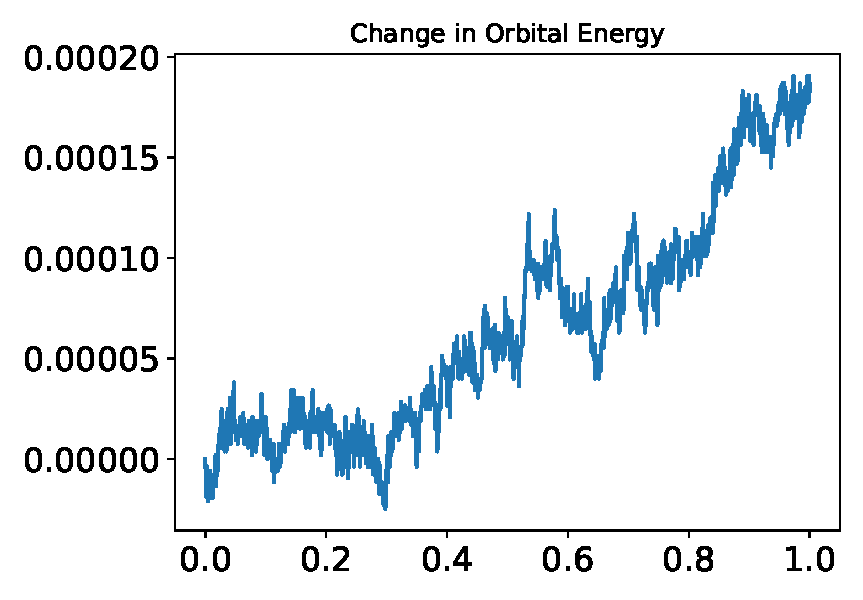
\includegraphics[width=0.8\textwidth]{AutoTeX/ChangeInRotationalAngularMomentumBalancedWheels}}\caption{Change in Rotational Angular Momentum BalancedWheels}\label{fig:ChangeInRotationalAngularMomentumBalancedWheels}\end{figure}
\begin{figure}[htbp]\centerline{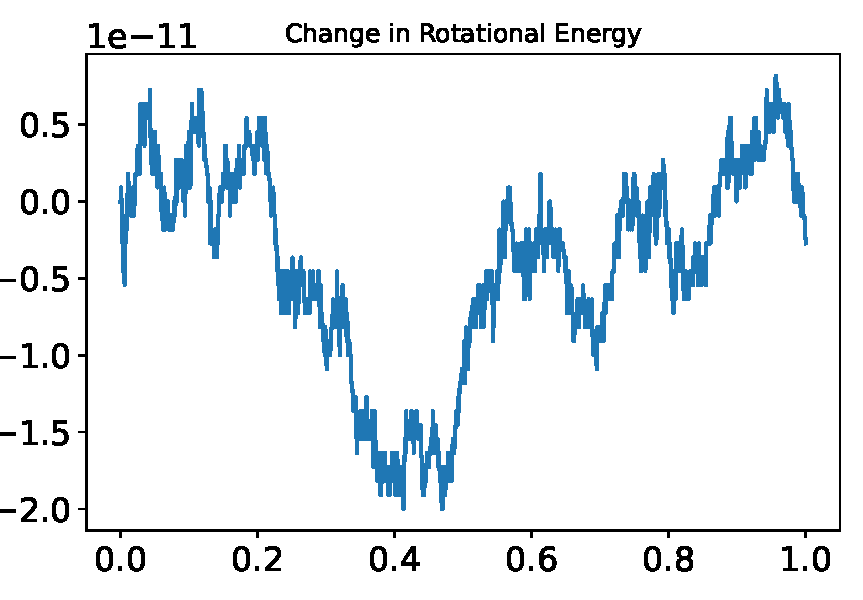
\includegraphics[width=0.80\textwidth]{AutoTeX/ChangeInRotationalEnergyBalancedWheels}}\caption{Change in Rotational Energy BalancedWheels}\label{fig:ChangeInRotationalEnergyBalancedWheels}\end{figure}

\clearpage

\subsection{Fully Coupled Jitter Scenario - Integrated Test Plots}

\begin{figure}[htbp]\centerline{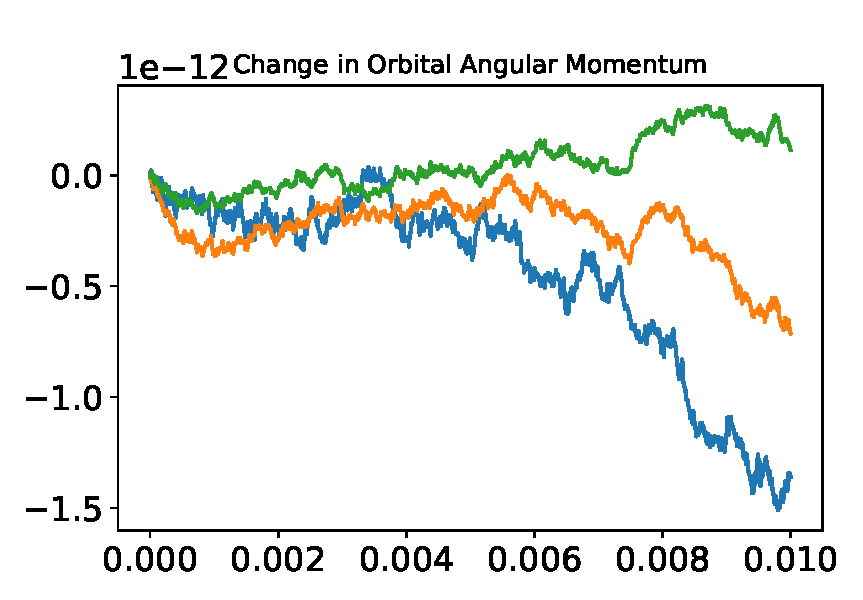
\includegraphics[width=0.8\textwidth]{AutoTeX/ChangeInOrbitalAngularMomentumJitterFullyCoupled}}\caption{Change in Orbital Angular Momentum JitterFullyCoupled}\label{fig:ChangeInOrbitalAngularMomentumJitterFullyCoupled}\end{figure}
\begin{figure}[htbp]\centerline{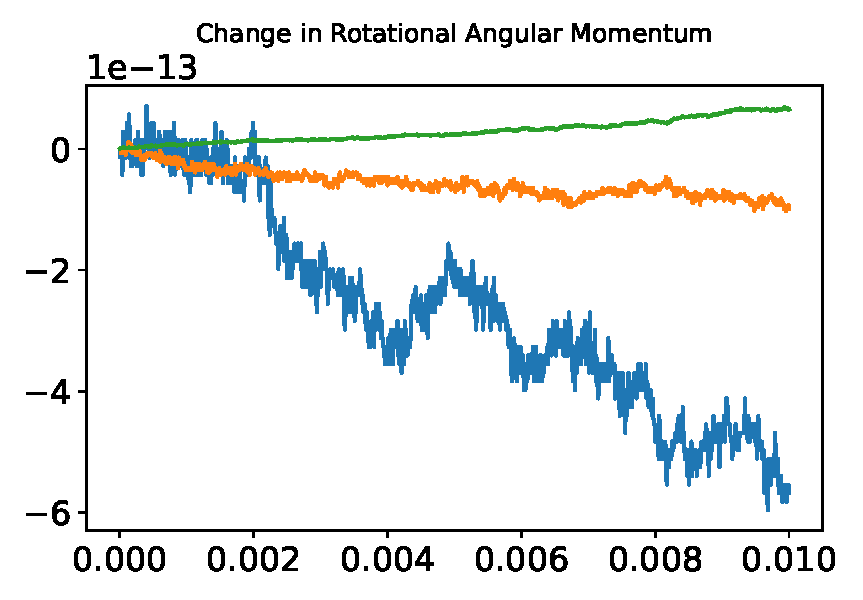
\includegraphics[width=0.8\textwidth]{AutoTeX/ChangeInOrbitalEnergyJitterFullyCoupled}}\caption{Change in Orbital Energy JitterFullyCoupled}\label{fig:ChangeInOrbitalEnergyJitterFullyCoupled}\end{figure}
\begin{figure}[htbp]\centerline{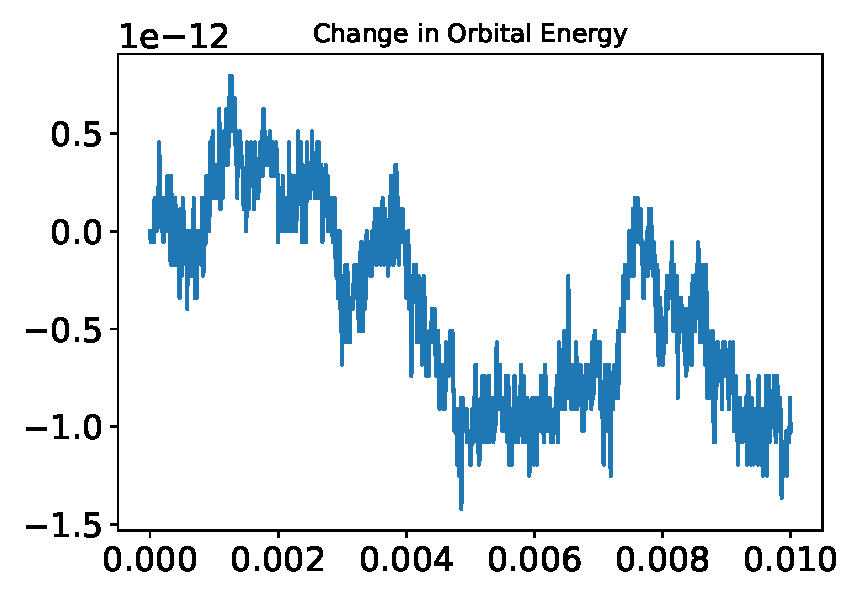
\includegraphics[width=0.80\textwidth]{AutoTeX/ChangeInRotationalAngularMomentumJitterFullyCoupled}}\caption{Change in Rotational Angular Momentum JitterFullyCoupled}\label{fig:ChangeInRotationalAngularMomentumJitterFullyCoupled}\end{figure}
\begin{figure}[htbp]\centerline{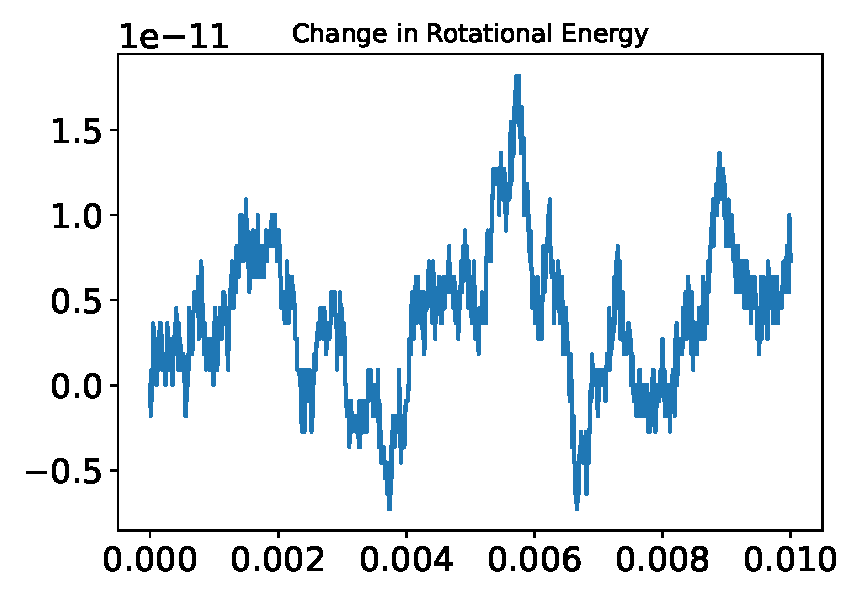
\includegraphics[width=0.80\textwidth]{AutoTeX/ChangeInRotationalEnergyJitterFullyCoupled}}\caption{Change in Rotational Energy JitterFullyCoupled}\label{fig:ChangeInRotationalEnergyJitterFullyCoupled}\end{figure}

\clearpage

\subsection{Fully Coupled Jitter with Gravity Scenario - Integrated Test Plots}

\begin{figure}[htbp]\centerline{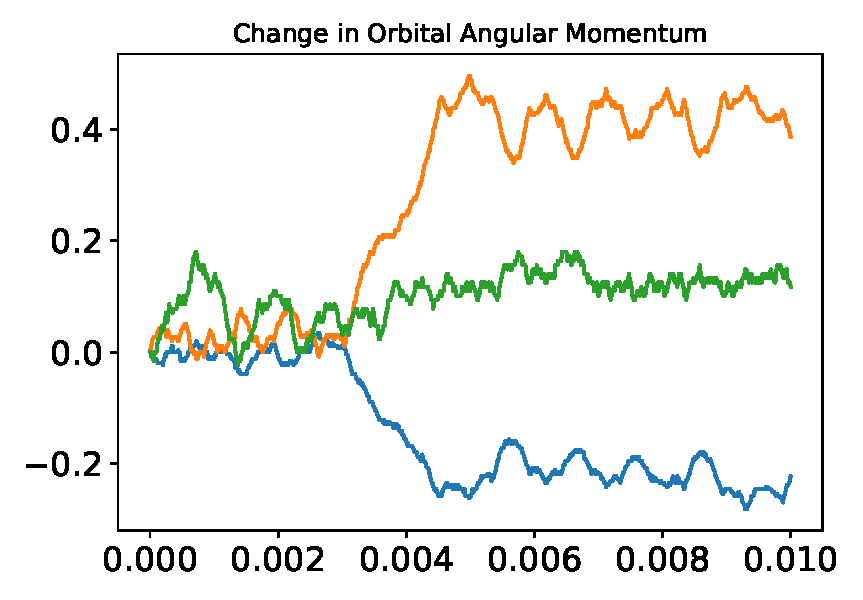
\includegraphics[width=0.80\textwidth]{AutoTeX/ChangeInOrbitalAngularMomentumJitterFullyCoupledGravity}}\caption{Change in Orbital Angular Momentum JitterFullyCoupledGravity}\label{fig:ChangeInOrbitalAngularMomentumJitterFullyCoupledGravity}\end{figure}
\begin{figure}[htbp]\centerline{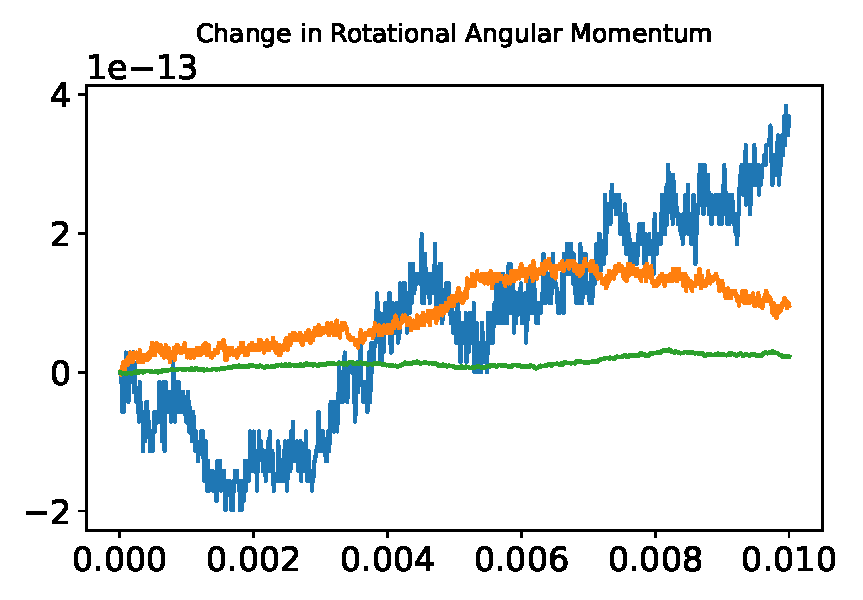
\includegraphics[width=0.80\textwidth]{AutoTeX/ChangeInOrbitalEnergyJitterFullyCoupledGravity}}\caption{Change in Orbital Energy JitterFullyCoupledGravity}\label{fig:ChangeInOrbitalEnergyJitterFullyCoupledGravity}\end{figure}
\begin{figure}[htbp]\centerline{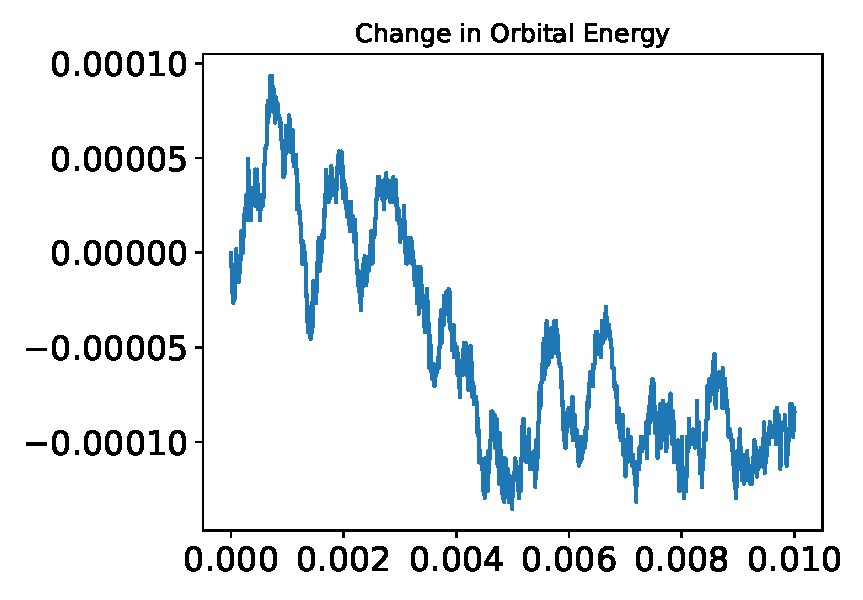
\includegraphics[width=0.80\textwidth]{AutoTeX/ChangeInRotationalAngularMomentumJitterFullyCoupledGravity}}\caption{Change in Rotational Angular Momentum JitterFullyCoupledGravity}\label{fig:ChangeInRotationalAngularMomentumJitterFullyCoupledGravity}\end{figure}

\clearpage

\subsection{Balanced Wheels, Simple Jitter, Fully Coupled Jitter and Fully Coupled Jitter with Gravity Tests Results}

\begin{table}[htbp]
	\caption{Test results.}
	\label{tab:results}
	\centering \fontsize{10}{10}\selectfont
	\begin{tabular}{c | c } % Column formatting, 
		\hline
		\textbf{Test} 				    & \textbf{Pass/Fail}  \\ \hline
		Balanced Wheels  & \textcolor{ForestGreen}{PASSED} \\
		Simple Jitter  & \textcolor{ForestGreen}{PASSED}   \\ 
		Fully Coupled Jitter & \textcolor{ForestGreen}{PASSED}  \\ 
		Fully Coupled Jitter + Gravity  & \textcolor{ForestGreen}{PASSED}  \\ \hline
	\end{tabular}
\end{table}

\clearpage
